\documentclass{beamer}

\usepackage{amsmath}
\usepackage{graphicx}
\usepackage{hyperref}

\usetheme{Madrid}
\usecolortheme{default}

\title{DeepSeek-V3 Technical Report}
\subtitle{Technical Report Overview}
\author{Ion Lipsiuc}
\institute{lipsiuci@tcd.ie}
\date{\today}

\begin{document}

\begin{frame}
    \titlepage
\end{frame}

\section{Introduction}

\begin{frame}
    \frametitle{Introduction}
    \begin{itemize}
        \item DeepSeek-V3 is a large Mixture of Experts (MoE) language model with 671 billion total parameters, of which 37 billion are activated per token.
        \item Key innovations:
              \begin{itemize}
                  \item Multi-Head Latent Attention (MLA) for efficient inference.
                  \item DeepSeekMoE architecture for cost-effective training.
                  \item Auxiliary-Loss-Free Load Balancing Strategy.
                  \item Multi-Token Prediction (MTP) training objective.
              \end{itemize}
        \item Pre-trained on 14.8 trillion tokens, achieving state-of-the-art performance.
        \item Training completed in 2.788 million H800 GPU hours, demonstrating remarkable stability.
    \end{itemize}
\end{frame}

\section{Multi-Head Latent Attention}

\begin{frame}
    \frametitle{Multi-Head Latent Attention}
    \begin{itemize}
        \item MLA reduces Key-Value (KV) cache during inference by compressing keys and values.
        \item Low-rank joint compression for attention keys and values.
        \item Formulation:
              \begin{equation*}
                  \mathbf{k}_{t,i}=\bigl[\mathbf{k}_{t,i}^C;\mathbf{k}_t^R\bigr],\quad\mathbf{v}_t^C=W^{UV}\mathbf{c}_t^{KV},
              \end{equation*}
              where:
              \begin{itemize}
                  \item $\mathbf{k}_{t,i}^C$: Compressed latent vector for keys.
                  \item $\mathbf{k}_t^R$: Decoupled key with Rotary Positional Embedding (RoPE).
                  \item $\mathbf{v}_t^C$: Compressed latent vector for values.
                  \item $\mathbf{c}_t^{KV}$: Latent representation used for both keys and values.
                  \item $W^{UV}$: A learnable projection matrix.
              \end{itemize}
        \item Only $\mathbf{c}_t^{KV}$ and $\mathbf{k}_t^R$ are cached, reducing memory usage significantly.
    \end{itemize}
\end{frame}

\begin{frame}
    \begin{figure}[htbp]
        \centering
        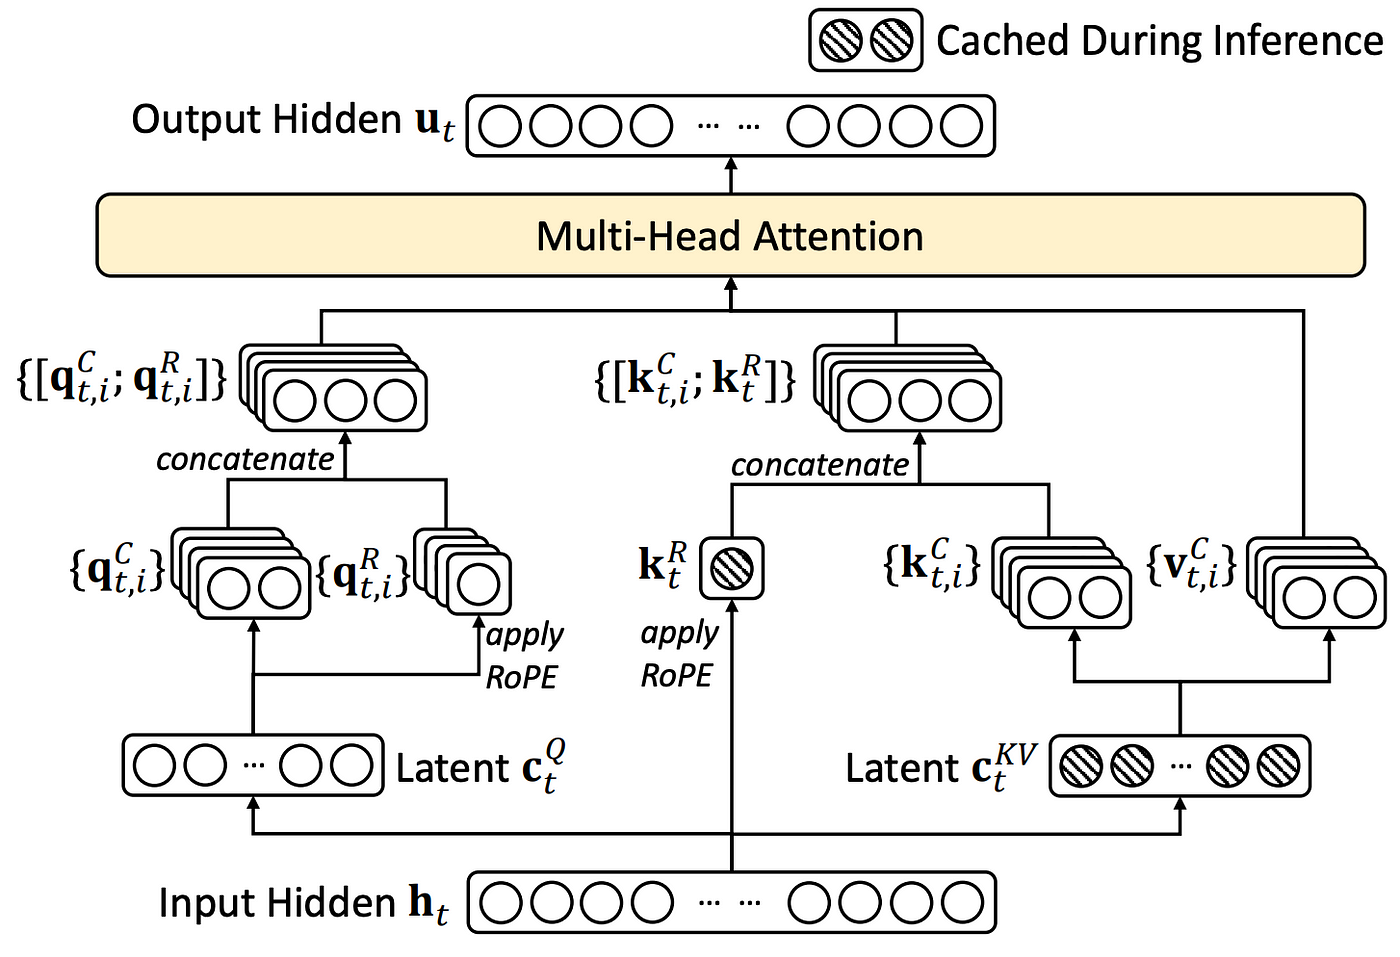
\includegraphics[scale=0.22031]{attachments/multi-head-latent-attention.png}\caption{Keys and values are compressed into latent representations, with a small set of components cached during inference to reduce memory usage.}
    \end{figure}
\end{frame}

\section{Mixture of Experts}

\begin{frame}
    \frametitle{Mixture of Experts}
    \begin{itemize}
        \item DeepSeekMoE uses a combination of shared experts and routed experts for efficiency.
        \item Formulation:
              \begin{equation*}
                  \mathbf{h}_t^\prime=\mathbf{u}_t+\sum_{i=1}^{N_s}\text{FFN}_i^{(s)}(\mathbf{u}_t)+\sum_{i=1}^{N_r}g_{i,t}\text{FFN}_i^{(r)(\mathbf{u}_{t})},
              \end{equation*}
              where:
              \begin{itemize}
                  \item $N_s$: Number of shared experts (applied to every token).
                  \item $N_r$: Number of routed experts (selectively applied to tokens).
                  \item $g_{i,t}$: Gating value for expert $i$ at time step $t$.
              \end{itemize}
        \item Auxiliary-loss-free load balancing ensures balanced expert usage without adding extra losses:
              \begin{equation*}
                  g_{i,t}^\prime=
                  \begin{cases}
                      s_{i,t}, & \text{if }s_{i,t}+b_i\in\text{Topk}(\{s_{j,t}+b_j\mid1\leq j\leq N_r\},K_r), \\
                      0,       & \text{otherwise}.
                  \end{cases}
              \end{equation*}
              Here $s_{i,t}$ is a raw score for expert $i$ and $b_i$ is a learned bias term.
    \end{itemize}
\end{frame}

\begin{frame}
    \begin{figure}[htbp]
        \centering
        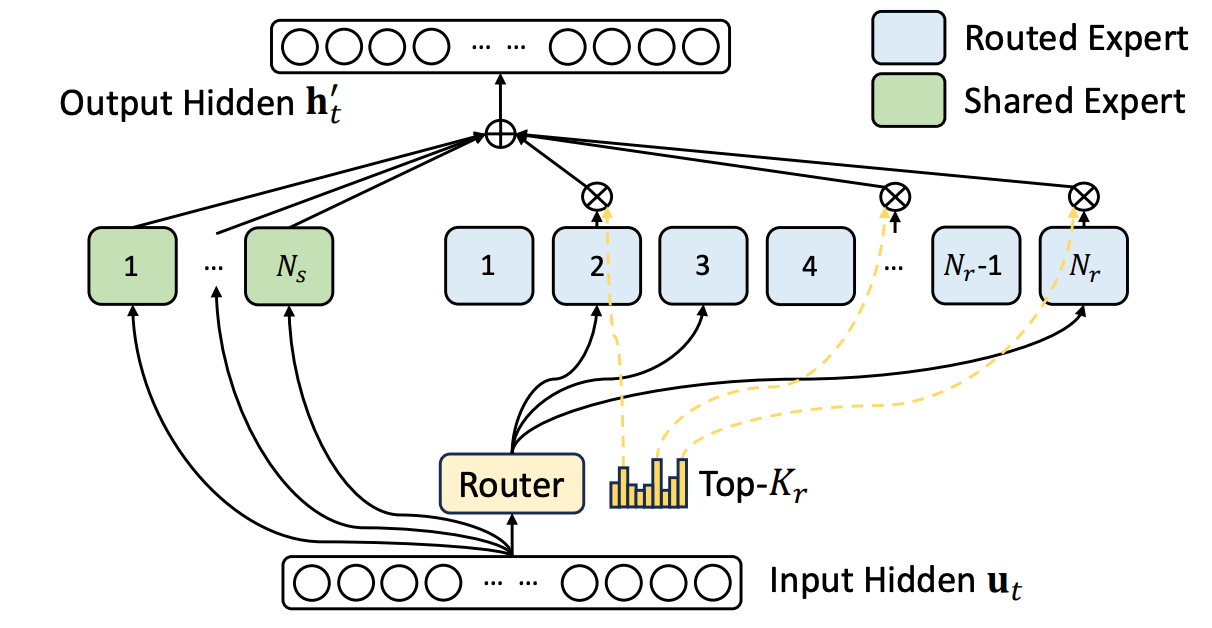
\includegraphics[scale=0.28145]{attachments/deepseekmoe.png}
        \caption{The router selects which experts (routed experts) to activate per token. Shared experts are always applied.}
    \end{figure}
\end{frame}

\section{Multi-Token Prediction}

\begin{frame}
    \frametitle{Multi-Token Prediction}
    \begin{itemize}
        \item MTP extends the prediction scope to multiple future tokens at once.
        \item Each module in MTP predicts one of the next several tokens, allowing partial parallelism.
        \item Formulation:
              \begin{equation*}
                  \mathbf{h}_i^k=M_k[\text{RMSNorm}(\mathbf{h}_i^{k-1});\text{RMSNorm}(\text{Emb}(t_{i+k}))],
              \end{equation*}
              where:
              \begin{itemize}
                  \item $\mathbf{h}_i^{k-1}$: Representation from the $(k-1)^\text{th}$ module.
                  \item $\text{Emb}(t_{i+k})$: Embedding of the $(i+k)^\text{th}$ token.
                  \item $M_k$: The $k^\text{th}$ MTP module (e.g., a Transformer block).
              \end{itemize}
        \item Overall training objective:
              \begin{equation*}
                  \mathcal{L}_\text{MTP}=\frac{\lambda}{D}\sum_{k=1}^D\mathcal{L}_\text{MTP}^k,
              \end{equation*}
              where $\mathcal{L}_\text{MTP}^k$ is the cross-entropy loss at depth $k$, and $D$ is the number of MTP modules.
    \end{itemize}
\end{frame}

\begin{frame}
    \begin{figure}[htbp]
        \centering
        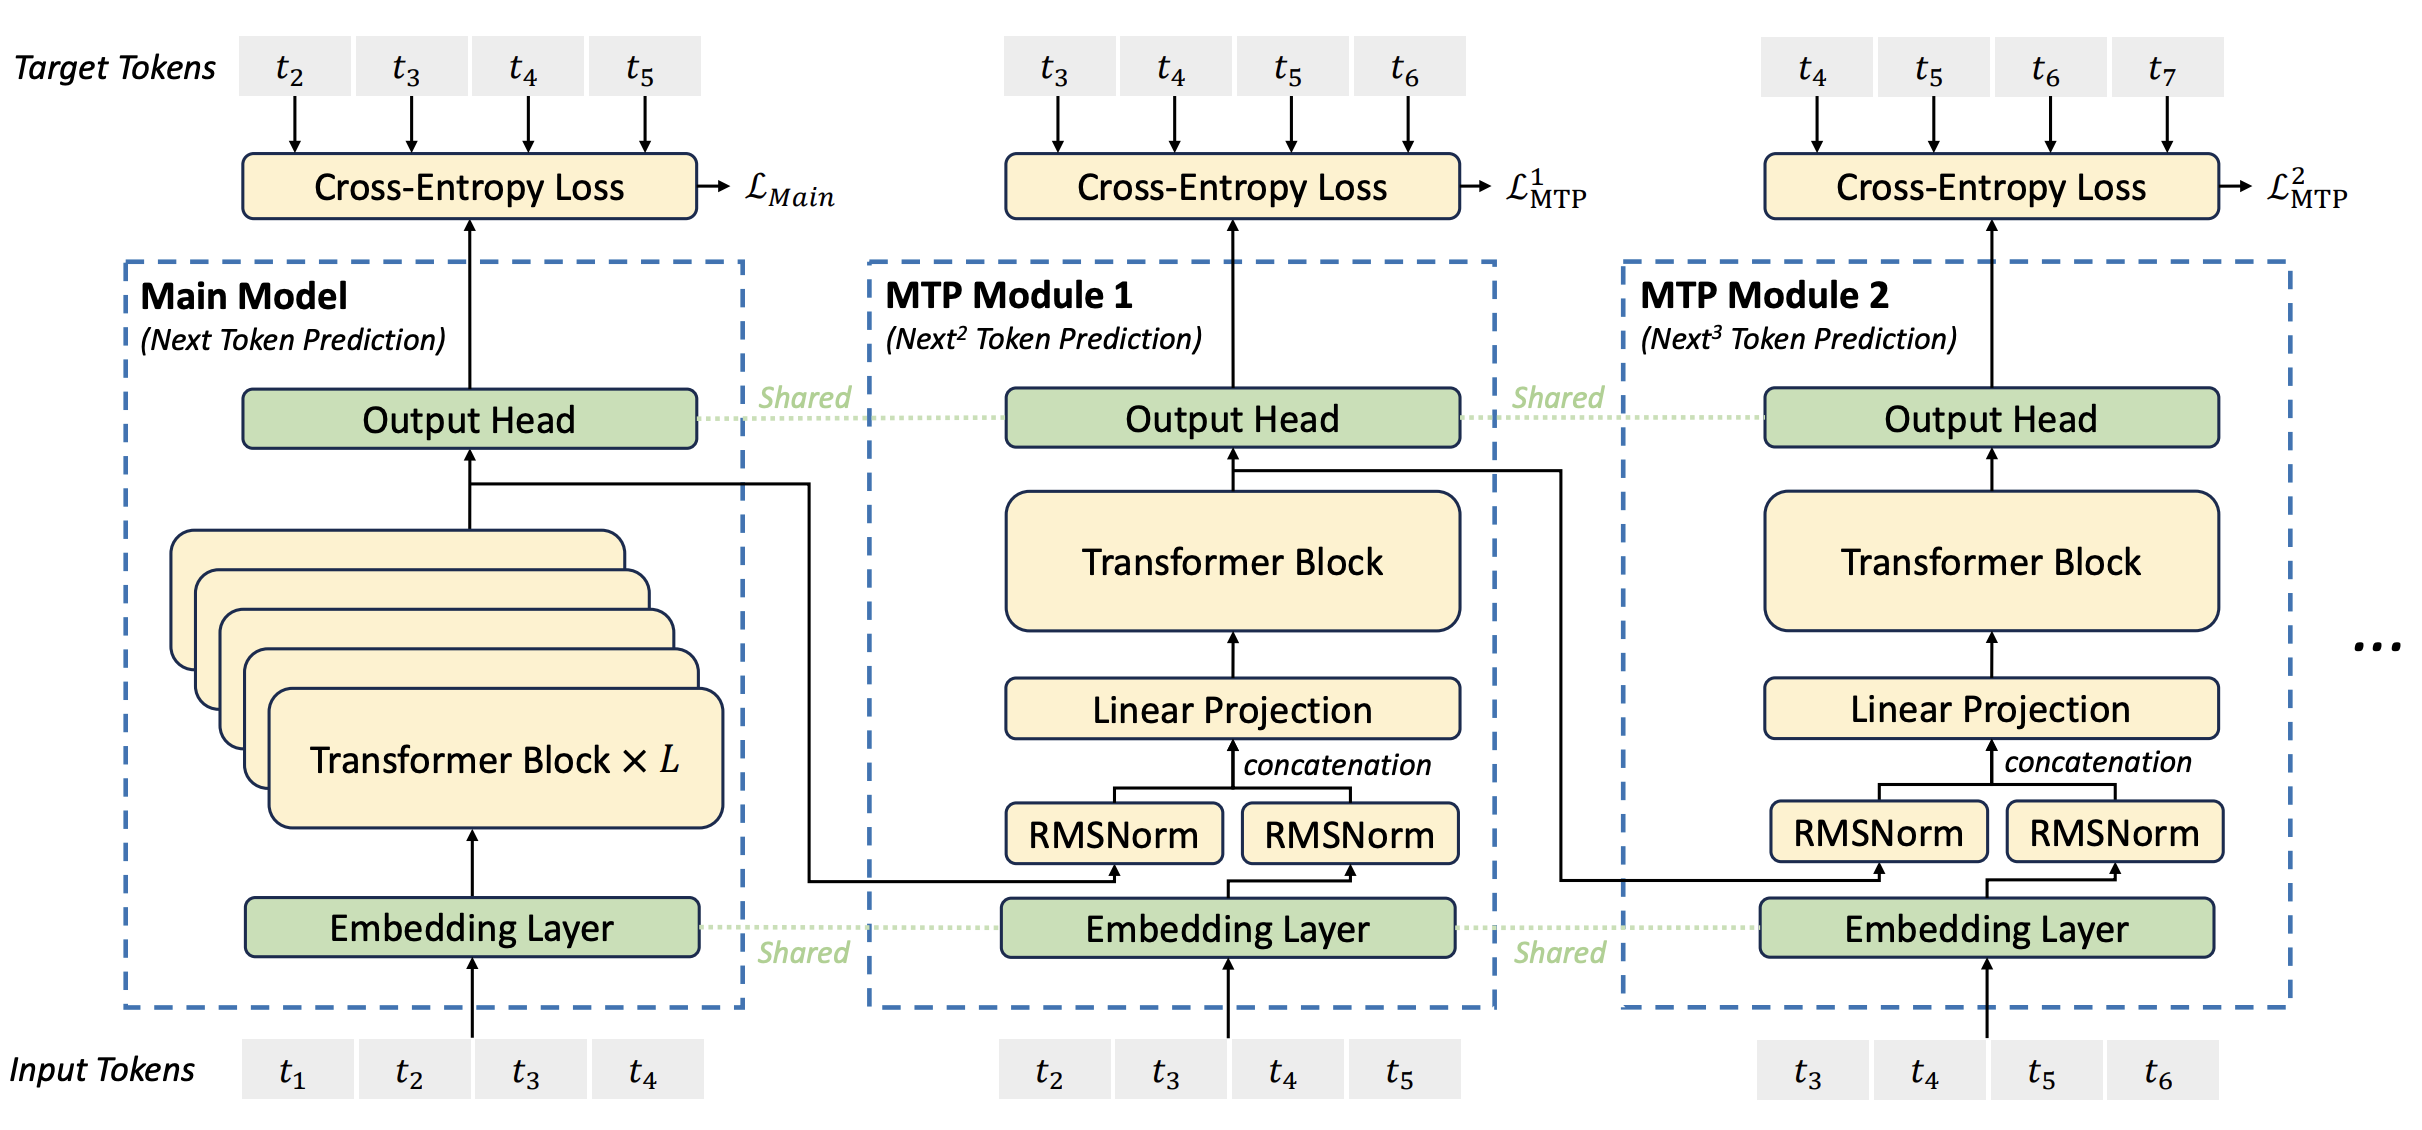
\includegraphics[scale=0.28168]{attachments/multi-token-prediction.png}
        \caption{Several modules predict future tokens in parallel, each focusing on a different next token.}
    \end{figure}
\end{frame}

\section{Compute Cluster and Training Framework}

\begin{frame}
    \frametitle{Compute Cluster and Training Framework}
    \begin{itemize}
        \item Trained on a cluster with \textbf{2048 NVIDIA H800 GPUs}.
        \item \textbf{DualPipe} algorithm for efficient pipeline parallelism:
              \begin{itemize}
                  \item Overlaps computation and communication.
                  \item Reduces pipeline bubbles and communication overhead.
              \end{itemize}
        \item \textbf{DualPipe scheduling}:
              \begin{itemize}
                  \item Divides chunks into attention, all-to-all dispatch, MLP, and all-to-all combine steps.
                  \item Overlaps forward and backward computation-communication phases.
              \end{itemize}
        \item \textbf{Efficient cross-node all-to-all communication}:
              \begin{itemize}
                  \item Utilizes InfiniBand (IB) and NVLink bandwidths.
                  \item Limits tokens to four nodes to reduce IB traffic.
              \end{itemize}
    \end{itemize}
\end{frame}

\begin{frame}
    \begin{figure}[htbp]
        \centering
        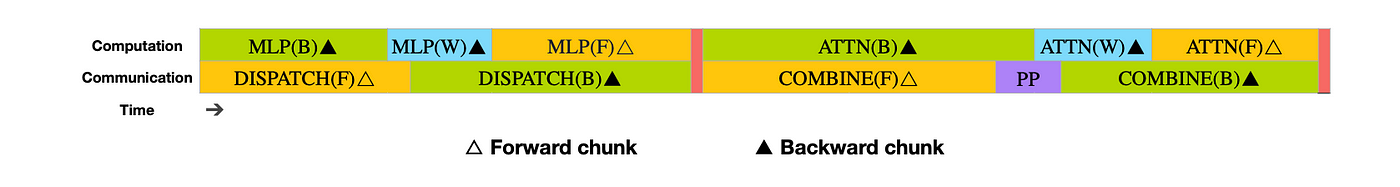
\includegraphics[scale=0.24365]{attachments/overlapping-strategy.png}
        \caption{Example of pipeline stages (attention, MLP, dispatch/collect steps) overlapping forward (colored blocks) and backward (triangles) phases.}
    \end{figure}
\end{frame}

\begin{frame}
    \begin{figure}[htbp]
        \centering
        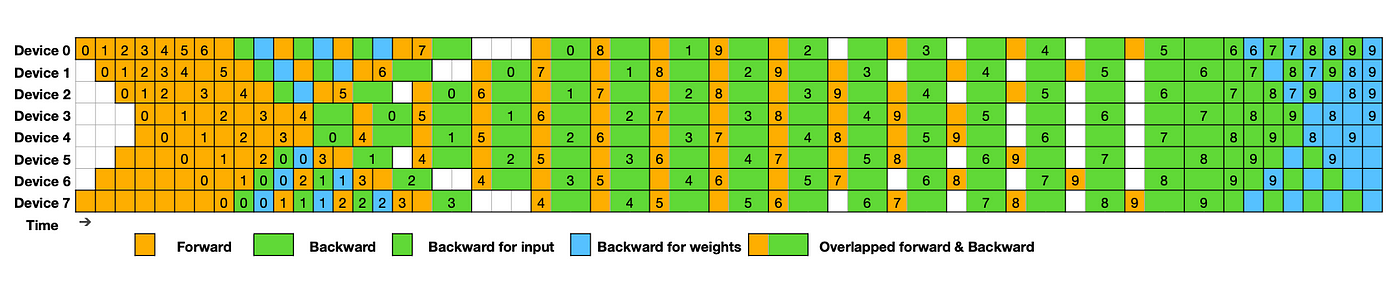
\includegraphics[scale=0.24365]{attachments/dualpipe-scheduling.png}
        \caption{This timeline illustrates how forward and backward passes are distributed across eight devices, with color-coded segments indicating computation or communication tasks.}
    \end{figure}
\end{frame}

\section{FP8 Training}

\begin{frame}
    \frametitle{FP8 Training}
    \begin{itemize}
        \item \textbf{FP8 mixed precision training framework}:
              \begin{itemize}
                  \item Most compute-intensive operations in FP8 for speed and reduced memory.
                  \item Key operations in higher precision (BF16 or FP32) to maintain numerical stability.
              \end{itemize}
        \item \textbf{Fine-grained quantization}:
              \begin{itemize}
                  \item Activations: 1x128 tile basis (small sub-blocks).
                  \item Weights: 128x128 block basis.
              \end{itemize}
        \item \textbf{Low-precision storage and communication}:
              \begin{itemize}
                  \item Activations cached in FP8 for the backward pass.
                  \item Optimizer states stored in BF16 to reduce memory usage.
              \end{itemize}
        \item Achieves high training efficiency with minimal precision loss.
    \end{itemize}
\end{frame}

\begin{frame}
    \begin{figure}[htbp]
        \centering
        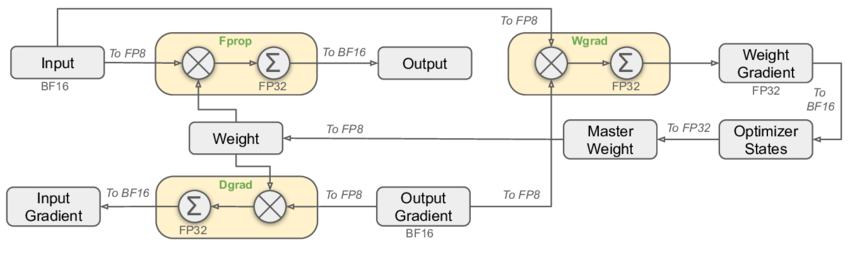
\includegraphics[scale=1.20394]{attachments/mixed-precision-training.png}
        \caption{The forward pass (Fprop) and backward pass (Dgrad, Wgrad) are done in FP8. A master copy of the weights is kept in BF16 or FP32 for numerical stability.}
    \end{figure}
\end{frame}

\section{Pre-Training}

\begin{frame}
    \frametitle{Pre-Training}
    \begin{itemize}
        \item Pre-trained on \textbf{14.8 trillion} high-quality tokens.
        \item \textbf{Two-stage context length extension}:
              \begin{itemize}
                  \item Stage 1: Extend context length to 32K.
                  \item Stage 2: Extend context length to 128K.
              \end{itemize}
        \item Remarkably stable training process:
              \begin{itemize}
                  \item No irrecoverable loss spikes or rollbacks.
              \end{itemize}
        \item Post-training includes:
              \begin{itemize}
                  \item \textbf{Supervised Fine-Tuning (SFT)}.
                  \item \textbf{Reinforcement Learning (RL)}.
                  \item \textbf{Distillation} from DeepSeek-R1 for better reasoning.
              \end{itemize}
    \end{itemize}
\end{frame}

\section{Conclusion}

\begin{frame}
    \frametitle{Conclusion}
    \begin{itemize}
        \item DeepSeek-V3 is a state-of-the-art open-source MoE model.
        \item Key innovations: \textbf{MLA}, \textbf{DeepSeekMoE}, \textbf{MTP}, and \textbf{FP8} training.
        \item Achieves high performance with economical training costs.
    \end{itemize}
\end{frame}

\end{document}
